\title{Advanced Topics in Programming Language - Duck Typing in Python}
\author{
        Tommaso Puccetti \\
                Studente presso Universita degli studi di Firenze
}
\date{\today}
\documentclass[12pt]{article}
\usepackage{graphicx}
\usepackage{hyperref}
\usepackage{listings}
\usepackage{jlcode}

\begin{document}
\maketitle
\tableofcontents
\listoftables
\listoffigures

\section{Possible references}
	\begin{itemize}
		\item \href{https://www.youtube.com/watch?v=fK5lcaNqdj4}{You Tube video};
		\item \href{https://hackernoon.com/python-duck-typing-or-automatic-interfaces-73988ec9037f}{Python duck typing (or automatic interfaces)- how change the dependecy injection};
		\item \href{https://medium.com/programming-hacks/duck-typing-in-python-6740aa72b301}{Simple example};
		\item \href{http://www.voidspace.org.uk/python/articles/duck_typing.shtml}{Something more technical};
		\item 
		\href{https://realpython.com/python-type-checking/}{Ultimate guide to Python's type checking;}
		\item
		\href{https://stackoverflow.com/questions/1517582/what-is-the-difference-between-statically-typed-and-dynamically-typed-languages}{Static vs Dynamic (Stack Overflow)}
		\item
		\href{https://wiki.python.org/moin/Why is Python a dynamic language and also a strongly typed language}{Why Python is dynamic and strongly typed}
		\item
		\href{https://android.jlelse.eu/magic-lies-here-statically-typed-vs-dynamically-typed-languages-d151c7f95e2b}{Maybe schematic overview on typechecking}
	\end{itemize}

\section{Questions}
	\begin{itemize}
		\item Are language that implement type inference always static ?
	\end{itemize}
\newpage
\section{Type checking: classification}
	\textbf{Type checking} is the process of verifying and enforces the typing rules of a language. In other words the \textbf{type checker} (the type checking algorithm of the language ) is used to prove the \textbf{type safety} of a program.\\
	Here the possible categories:
	\begin{itemize}
		\item Dynamic vs. Static;
		\item Explicit vs Implicit;
		\item Weakly vs Strongly
	\end{itemize}

	\begin{figure}[h!]
		\centering
		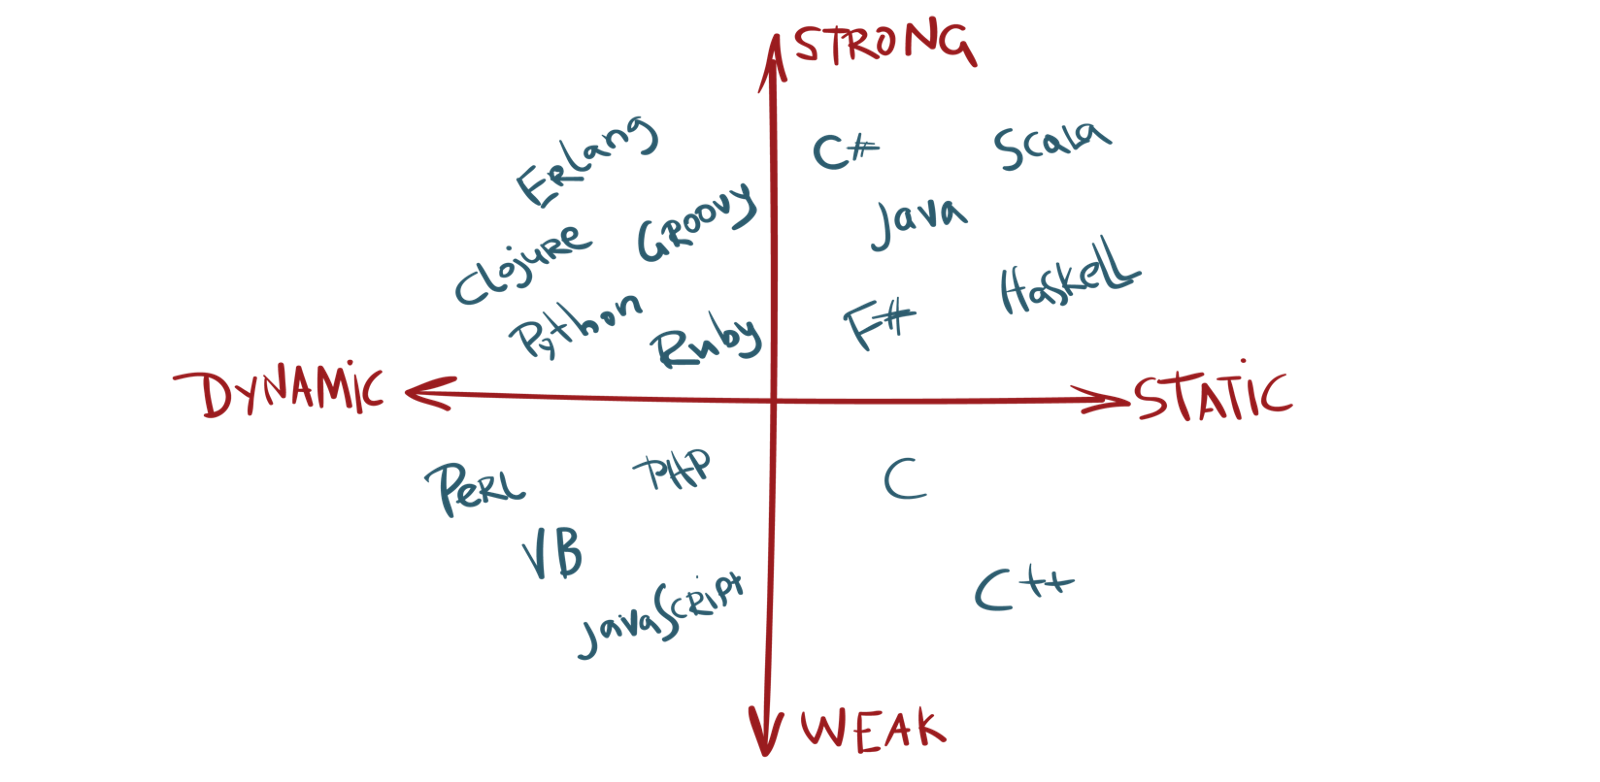
\includegraphics[scale=0.20]{img/classification.png}
	\end{figure}

	\subsection{Static type checking}
		Is the process of verifying the type safety of a program based on the analysis of a program text.  If a program passes a static type checker, then the program is guaranteed to satisfy some set of type safety properties for all possible inputs \textit{\textbf{(Wikipedia)}}.\\
		A language is statically typed if the type of a variable is known at compile time. For some languages this means that you as the programmer must specify what type each variable is (e.g.: Java, C, C++); other languages offer some form of type inference, the capability of the type system to deduce the type of a variable \textit{\textbf{(Stack Overflow)}};\\
		A language is statically-typed if the type of a variable is known at compile-time instead of at run-time. Common examples of statically-typed languages include Java, C, C++, FORTRAN, Pascal and Scala. \textbf{\textit{(Schematic overview)}};\\
		
		\begin{figure}[h!]
			\centering
			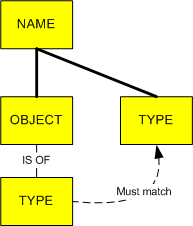
\includegraphics[scale=0.60]{img/static.png}
		\end{figure}
	
		\subsubsection{Example}	
			Here a java example: 
			\begin{lstlisting}[language=Java]
				int variable;
				variable = 10;
				variable = "ten";
			\end{lstlisting}
			It causes a compilation error:
			\begin{lstlisting}
				INSERIRE ERRORE DI COMPILAZIONE
			\end{lstlisting}
			
		\subsubsection{Advantages}
			\begin{itemize}
				\item  A large class of errors are caught in the early stage of development process;
				\item Static typing usually results in compiled code that executes more quickly because when the compiler knows the exact data types that are in use, it can produce optimized machine code.
			\end{itemize}
			
	\subsection{Dynamic type checking}
		Is the process of verifying the type safety of a program at runtime. It may cause a program to fail at runtime \textit{\textbf{(Wikipedia)}}.\\
		A language is dynamically typed if the type is associated with run-time values, and not named variables/fields/etc. This means that you as a programmer can write a little quicker because you do not have to specify types every time (unless using a statically-typed language with type inference) \textit{\textbf{(Stack Overflow)}}.\\
		In Dynamically typed languages, variables are bound to objects at run-time by means of assignment statements, and it is possible to bind the same variables to objects of different types during the execution of the program.
		Dynamic type checking typically results in less optimized code than static type checking. It also includes the possibility of run time type errors and forces run time checks to occur for every execution of the program (instead of just at compile-time) (\textbf{\textit{Schematic overview}}).\\
		
		\begin{figure}[h!]
			\centering
			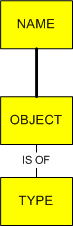
\includegraphics[scale=0.60]{img/dynamic.png}
		\end{figure}
	
		\subsubsection{Example}
			\begin{lstlisting}
				variable = 10
				variable = "ten"
			\end{lstlisting}
		
		\subsubsection{Advantages}
			\begin{itemize}
				\item Implementations of dynamically type-checked languages generally associate each run time object with a type tag (i.e., a reference to a type) containing its type information. This run-time type information (RTTI) can also be used to implement dynamic dispatch, late binding, down-casting, reflection, and similar features;
				\item The absence of a separate compilation step means that you don’t have to wait for the compiler to finish before you can test your code changes. This makes the debug cycle much shorter and less cumbersome.
			\end{itemize}
			
		CAPIRE SE SONO SOTTO CATEGORIE DI STATIC O DISTINZIONE PIU GENERALE 
	\subsection{Explicitly typed}
		Each variables is annotaded in source code with type's information. In this case the \textit{type check is simple but the language is more difficult} (from the programmers point of view).
			
	\subsection{Implicitly typed (inference)}
		The data types of source code are automatically detected. It is also rederred as \textbf{type inference}. The language \textit{is easier but the type check algorithm is far more complex}.
	\subsection{Strongly typed}
		A strongly-typed language is one in which variables are bound to specific data types, and will result in type errors if types do not match up as expected in the expression regardless of when type checking occurs. (\textbf{\textit{Schematic overview}})\\
		\subsubsection{Example}
			\begin{lstlisting}
				variable1 = 10
				variable2 = "ten"
				variable3 = variable1 + variable2
			\end{lstlisting}
	\subsection{Weakly typed} 
		A weakly-typed language on the other hand is a language in which variables are not bound to a specific data type; they still have a type, but type safety constraints are lower compared to strongly-typed languages.\\
			\begin{lstlisting}
				$temp = "ten"; 
				$temp = $temp + 10; // no error caused
				echo $temp;
			\end{lstlisting}
			
			
		
	
		\subsection{Example: type inference vs. dynamic typing}
			These two kind of typings could be confused. Here an example to clarify the differences:

			\begin{lstlisting}[language=Python]
				var1 = 10
				var2 = "astring"
				var3 = var1 + var2
			\end{lstlisting}
			
			\begin{enumerate}
				\item In \textbf{dynamically typed} language this code run without errors: at runtime the \textit{var1} is forced to be a string and the result is \textit{"10astring"};
				\item By the other side, in \textbf{inferred type language} the compiler \textit{throw an error}.
			\end{enumerate}
\newpage
\section{Python type checking}
		
		Python is \textbf{dynamic}: objects have a type but it is determined at runtime. \\
		\textit{It rarely uses what it knows to limit variable usage.}
		
		\begin{lstlisting}
			if False:
				print(10+"ten") 
			else:
				print(10+10)
		\end{lstlisting}
		
		The first branch never execute, so the type checking ignore the type incongruency.\\
		Let's try to run:
		
		\begin{lstlisting}
			print(10+"ten")
		\end{lstlisting}
		
		Once executed the type check raise a type error:
		
		\begin{lstlisting}
			TypeError: unsupported operand type(s) for +: 'int' and 'str'
		\end{lstlisting}
		
		Another consequnce is that programmers are \textbf{free to bind the same names (variables) to different objects with a different type}. Then the following statements are perfectly legal:
		
		\begin{lstlisting}
			variable = 10
			variable = "ten"
		\end{lstlisting}
		
		
		
		
		
		
	
		
		






		
\end{document}